\documentclass{beamer}
\usetheme{Amsterdam}
\setbeamertemplate{navigation symbols}{}
%	
\usepackage{subfig}
\usepackage{amsmath, amsthm, amssymb}
\usepackage{float}
\usepackage{rotating}
\usepackage{graphicx}
\usepackage{longtable}
\usepackage{xcolor}
\usepackage{bm}
\usepackage{tikz}
\usepackage{epstopdf}
\usetikzlibrary{shapes}
\tikzset{My Arrow Style/.style={single arrow, fill=red!50, anchor=base, align=center,text width=.5cm,rotate =270}}
\newcommand{\MyArrow}[2][]{\tikz[baseline] \node [My Arrow Style,#1] {#2};}
\tikzset{My 2Arrow Style/.style={single arrow, fill=red!50, anchor=base, align=center,text width=.5cm,rotate =90}}
\newcommand{\MyArrowUp}[2][]{\tikz[baseline] \node [My 2Arrow Style,#1] {#2};}
\newcommand{\bmat}{\begin{matrix}}
\newcommand{\emat}{\end{matrix}}
\newcommand{\EE}{\mathbb E}

\newtheorem{acknowledgement}[theorem]{Acknowledgement}
\newtheorem{algorithm}[theorem]{Algorithm}
\newtheorem{assumption}{Assumption}
\newtheorem{axiom}{Axiom}
\newtheorem{case}[theorem]{Case}
\newtheorem{claim}[theorem]{Claim}
\newtheorem{conclusion}[theorem]{Conclusion}
\newtheorem{condition}[theorem]{Condition}
\newtheorem{conjecture}{Conjecture}
\newtheorem{criterion}[theorem]{Criterion}
\newtheorem{proposition}{Proposition}
\newtheorem{summary}[theorem]{Summary}
\newtheorem{exercise}{Exercise}
\newtheorem{notation}{Notation}
\newtheorem{remark}{Remark}
\newcommand{\barB}{{\overline B}}
\newcommand{\barC}{{\overline C}}
\newcommand{\pbar}{{\overline p}}
\newcommand{\bbar}{{\overline b}}
\newcommand{\mubar}{{\overline \mu}}
\newcommand{\var}{{\text{var}}}
\newcommand{\cov}{{\text{cov}}}

\epstopdfDeclareGraphicsRule{.tiff}{png}{.png}{%
  convert #1 \OutputFile         
}
\title{Linearization of Policy Functions with Incomplete Markets}
\begin{document}
\maketitle
\section{Steady State Payoff Structures}
\subsection{}
\begin{frame}
	\frametitle{The Problem}
	Our problem can be written recursively as follows
	\[
	V(b) = \max_{c(s),l(s),b'(s)}\sum_s \Pi(s)\left[ c(s) - \frac{l(s)^{1+\gamma}}{1+\gamma}+ \beta V(b'(s)) \right]
\]subject to the constraints
\begin{subequations}
\begin{align}\label{eq.imp}
	c(s) - l(s)^{1+\gamma}  + b'(s)  = \frac{p_s b}{\beta}\\
	c(s) + g_s  \leq l(s)\label{eq.res}
\end{align}
\end{subequations}
\begin{itemize}
	\item We can show that this problem is convex and $V(b)$ is concave.
	\item Let $\mu = V'(b)$, then there exists a mapping $b(\mu)$ that maps the multiplier on the implementability constraint into government debt.
\end{itemize}
\end{frame}
\begin{frame}
	\frametitle{First Order Conditions}
	\begin{itemize}
		\item  The first order conditions can be written succinctly as finding a function $b(\mu)$ such that the following system of equations can be solved for all $\mu$.
		\begin{align}\label{eq.lin_imp}
	\frac{b(\mu)p_s}{\beta \EE p} = I(\mu'(s)) - g_s +b(\mu'(s))\\
	\mu = \frac{\EE\mu' p}{\EE p}\label{eq.lin_mart}
\end{align} 
	\item Where 
	\[
		I(\mu) = (1-\tau(\mu))^\frac1\gamma\tau(\mu) \text{  and  } \tau(\mu) = \frac{\gamma\mu}{(1+\gamma)\mu-1}
	\]
	\end{itemize}
\end{frame}

\begin{frame}
	\frametitle{Payoffs with a Steay State}
	\begin{itemize}
		\item  We wish to find payoff $\overline p_s$ (normalized so that $\EE\pbar = 1$) such that the policy functions $\mu'(\mubar,s) = \mubar$ is optimal.
		\item  Plugging this into our implementability constraint we see
		\[
			\frac{\bbar \pbar_s}{\beta} = I(\mubar) - g_s + \bbar
		\]
		\item  Subtracting $s'$ from $s$ we have
		\[
			\frac{\bbar(\pbar_s-\pbar_{s'})}{\beta} = g_{s'}-g_{s'}
		\]or 
		\[
			\pbar_{s} - \pbar_{s'} = \frac{-\beta}{\bbar}(g_{s'} - g_s)
		\]
	\end{itemize}
\end{frame}

\begin{frame}
	\frametitle{Payoffs with a Steady State}
	\begin{itemize}
		\item  The steady state level of debt associated with $\mubar$ is 
		\[
			\bbar(\mubar) = \frac{\beta}{1-\beta}\left( I(\mubar) - \EE g\right)
		\]
		\item  With both of these equations we can construct the payoff vector associated with a steady state multiplier $\mubar$
		\[
			\pbar(\mubar)_s = 1-\frac{\beta}{\bbar(\mubar)}(g_s-\EE g)
		\]
		\item  A key element to note here is that if $\pbar_s$ has a complete markets steady state then $\pbar$ is perfectly correlated with $g$.
	\end{itemize}
\end{frame}
\section{Linearizing around the Steady State}
\subsection{}
\begin{frame}
	\frametitle{Larger State Space}
	\begin{itemize}
		\item Until this point we have considered our policy rules $\mu'(s,\mu)$ and $b(\mu)$ to be solely functions of $\mu$.
		\item These functions must satisfy
		\[
			F(\mu',b,\mu) = \vec 0
		\]where $F$ was our first order conditions above.
		\item  In truth, these policy functions  are also functions of the payoff vector $p$ so $\mu'(s,\mu,p)$ and $b'(\mu,p)$.
		\item  Moreover, we know that at $\mubar,\pbar(\mubar)$  we have
		\[
			F(\mu',b,\mubar,\pbar(\mubar)) = 0
		\]as well as  $\mu'(s,\mubar,\pbar(\mubar)) = \mubar$ and $\bbar(\mubar,\pbar(\mubar)) = \bbar(\mubar)$
	\end{itemize}
\end{frame}
\begin{frame}
\begin{center}
	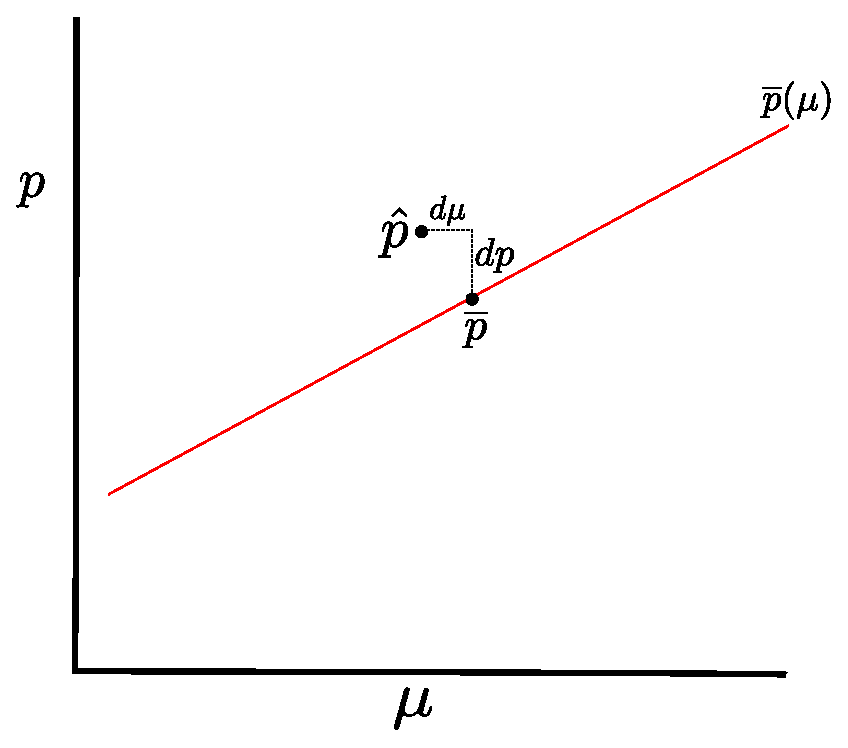
\includegraphics[width=3.5in]{Images/state_space.eps}
\end{center}
\end{frame}
\begin{frame}
	\frametitle{Linearize with Respect to $\mu$}
	\begin{itemize}
		\item  Differentiating the first order conditions with respect to $\mu$ around $(\mubar,\pbar)$ we obtain
		\[
			\frac{\pbar_s}{\beta}\frac{\partial b}{\partial \mu} = \left[I'(\mubar)+\frac{\partial b}{\partial \mu}\right]\frac{\partial \mu'(s)}{\partial \mu},
		\]and 
		\[
			1 = \sum_{s'}\Pi_{s'}\pbar_{s'}\frac{\partial\mu'(s')}{\partial \mu}
		\]
		\item  Applying $\sum_{s'}\Pi_{s'}\pbar_{s'}\cdot$ to the first equation we get
		\[
			\frac{\partial b}{\partial\mu} = \frac{I'(\mubar)}{\frac{\EE\pbar^2}{\beta} - 1}\text{  and }\frac{\partial\mu'(s)}{\partial \mu} = \frac{p_s}{\EE\pbar^2} 
		\]
	\end{itemize}
\end{frame}

\begin{frame}
	\frametitle{Linearize with Respect to $p$}
	\begin{itemize}
		\item  Differentiating with respect to $p_s$ around $(\mubar,\pbar)$ we get
		\begin{equation}\label{eq.dimp_dps}
			\frac{\pbar_{s'}}{\beta}\frac{\partial b}{\partial p_s} + 1_{s,s'}\frac{\bbar}{\beta} - \frac{\Pi_s\bbar\pbar_{s'}}{\beta} = \left[I'(\mubar) + \frac{\partial b}{\partial \mu}\right]\frac{\partial \mu'(s')}{\partial p_s}
		\end{equation}and 
		\[
			0 = \sum_{s'}\Pi_{s'}\pbar_{s'}\frac{\partial\mu'(s')}{\partial p_s}
		\]
		\item  The same trick as last slide applied to equation \eqref{eq.dimp_dps} gives
		\begin{equation}
			\frac{\partial b}{\partial p_s} = \Pi_s\bbar \frac{\EE\pbar^2-\pbar_s}{\EE\pbar^2}
		\end{equation}and
		\begin{equation}
	\frac{\partial \mu'(s')}{\partial p_s} = \frac{\bbar}{\beta\left[I '(\mubar) + \frac{\partial b}{\partial \mu}\right]}\left(1_{s,s'}-\frac{\Pi_s\pbar_s\pbar_{s'}}{\EE\pbar^2}\right)
\end{equation}
	\end{itemize}
\end{frame}

\section{Ergodic Distriubtion of the Linearized System}
\subsection{}
\begin{frame}
	\frametitle{Linearized system} 
	\begin{itemize}
		\item  For a given $p_s$ near $\pbar$ we can construct a linearized system
		\[
			\hat\mu_{t+1} = B\hat \mu_t + C
		\]where $\hat\mu = \mu_t -\mubar$ and $B$ and $C$ are random.
		\item  $B$ is just 
		\[
			B_{s'} = \frac{\partial \mu'(s')}{\partial \mu}
		\]
		\item While $C$ is given by
		\[
			C_{s'} = \sum_s \frac{\partial \mu'(s')}{\partial p_s}(p_s-\pbar_s)
		\]
	\end{itemize}
\end{frame}

\begin{frame}
	\frametitle{Ergodic Distribution}
	\begin{itemize}
		\item  With a little algebra we can characterize the moments of the ergodic distribution of $\hat \mu$.
		\item  Specifically we obtain that 
		\[
			\EE\hat\mu = \frac{\barC}{1-\barB}
		\]where $\barC = \sum_{s'} C_{s'}\Pi_{s'}$ and $\barB = \sum_{s'}\Pi_{s'} B_{s'}$
		\item The variance of the ergodic distribution is given by
		\[
			\sigma_{\hat\mu}^2 = \frac{\sigma_B^2(\EE\hat\mu)^2 + \sigma_{BC}\EE\hat\mu + \sigma_C^2}{1-\barB^2-\sigma_B^2}
		\]where $\sigma_B^2$, $\sigma_C^2$ and $\sigma_{BC}$ are the variance and covariance of $B$ and $C$ respectively
	\end{itemize}
\end{frame}
\section{The Best $\pbar$}
\subsection{}
\begin{frame}
	\frametitle{A Guess}
	\begin{itemize}
		\item  Given that we can approximate around any $(\mubar,\pbar)$ a natural question is if we want to approximate the solution for some $p$, with $\EE p = 1$, what is the best point to linearize around?
		\item  A natural answer is that we want to minimize the distance between $p$ and $\pbar$ given by
		\[
			\| p- \pbar\|^2 = \sum_{s} \Pi_s (p_s-\pbar_s)^2
		\]
		\item  Thus we wish to choose $\mubar,\pbar(\mubar)$ to minimize
		\[
			\|p-\pbar(\mubar)\|^2
		\]
		\item  We can show that choosing the point gives us additional benefits.
	\end{itemize}
\end{frame}

\begin{frame}
	\frametitle{A Property of the Minimizer}
	\begin{itemize}
		\item Taking the first order condition of the minimization problem we get 
		\[
			2\sum_{s'}\Pi_s'( p_{s'}-\pbar(\mubar)_{s'}) \pbar'(\mubar)_{s'} = 0
		\]
		\item  We noted before that $\pbar$ is a straight line in $\mathbb R^S$, thus $\pbar'(\mubar)\propto\pbar-1$.
		\item  Thus
		\begin{equation}
	\begin{split}
		0 &= \sum_{s'}\Pi_{s'}( p_{s'} - \pbar(\mubar)_{s'})(\pbar(\mubar)_{s'}-1)\\
		&= -\sum_{s'}\Pi_{s'}( p_{s'}-\pbar(\mubar)_{s'}) + \sum_{s'}\Pi_{s'}( p_{s'}-\pbar(\mubar)_{s'})\pbar(\mubar)_{s'}\\
		&= \sum_{s'}\Pi_{s'}( p_{s'}-\pbar(\mubar)_{s'})\pbar(\mubar)_{s'}\\
		&=\EE\left[( p-\pbar(\mubar))\pbar(\mubar)\right]
	\end{split}
\end{equation} 
	\end{itemize}
\end{frame}

\begin{frame}
	\frametitle{Mean of the Ergodic Distribution}
	\begin{itemize}
		\item  Using our formula for $C$ we have
		\begin{equation}
\begin{split}
	\barC &= \sum_s\left\{\frac{\bbar}{\beta\left[I'(\mubar)+\frac{\partial b}{\partial\mu}\right]}\left(\Pi_s - \frac{\Pi_s\pbar_s}{\EE\pbar^2}\right)(\hat p_s-\pbar_s)\right\}\\
	&=\frac{\bbar}{\beta\left[I'(\mubar)+\frac{\partial b}{\partial\mu}\right]}\left(\EE(\hat p-\pbar) -\frac{\EE\left[(\hat p-\pbar)\pbar\right]}{\EE\pbar^2}\right)\\
	&= 0 
\end{split}
\end{equation}
		\item  Thus we have that 
		\[
			\EE\hat\mu = \frac{\barC}{1-\barB}  = 0
		\]
		\item Thus the linearized system will have the same mean for $\mu$, $\mubar$, as the closest approximating steady state payoff structure.
	\end{itemize}
\end{frame}

\begin{frame}
	\begin{center}
		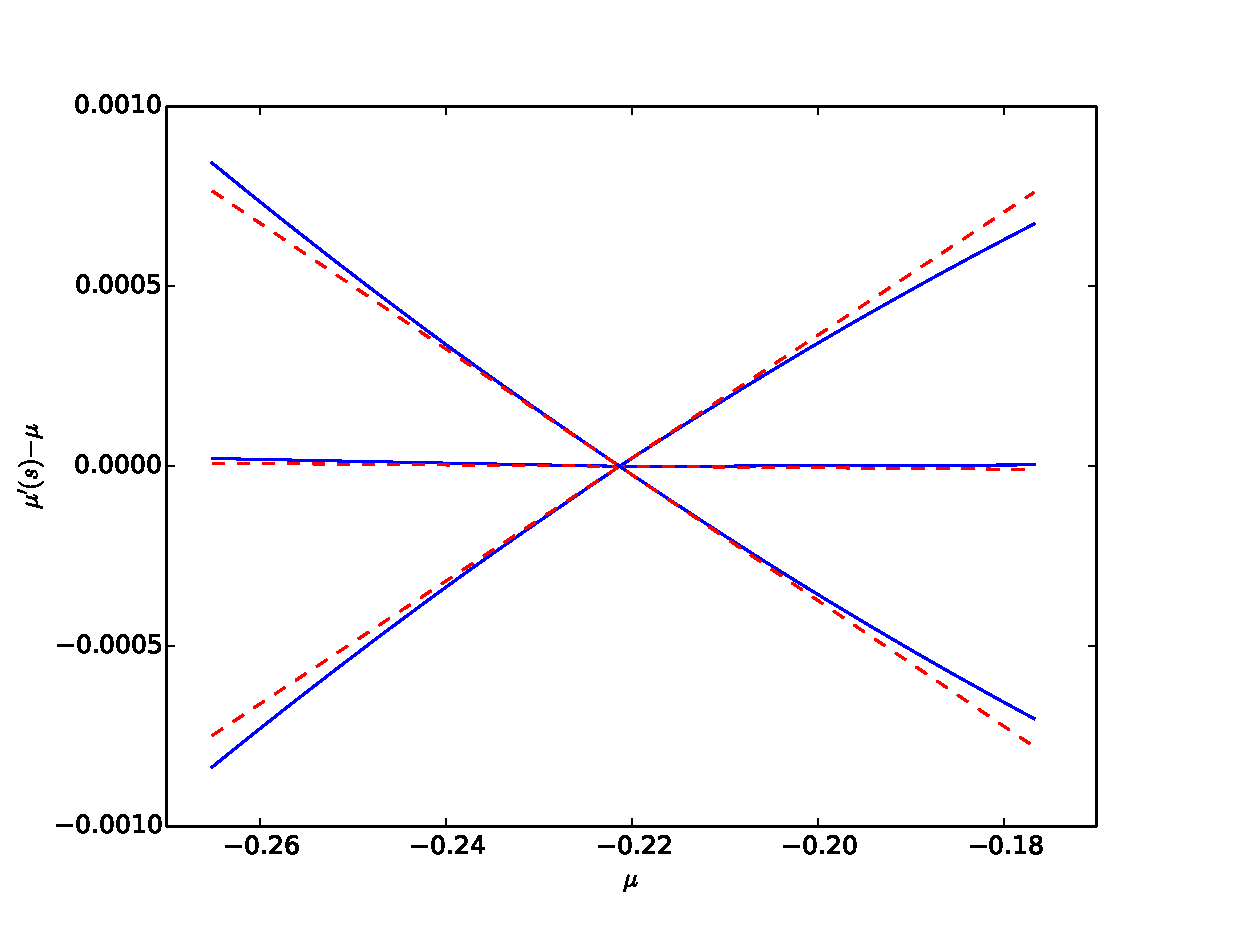
\includegraphics[width = 4.2in]{Images/lin1.eps}
	\end{center}
\end{frame}

\begin{frame}
	\begin{center}
		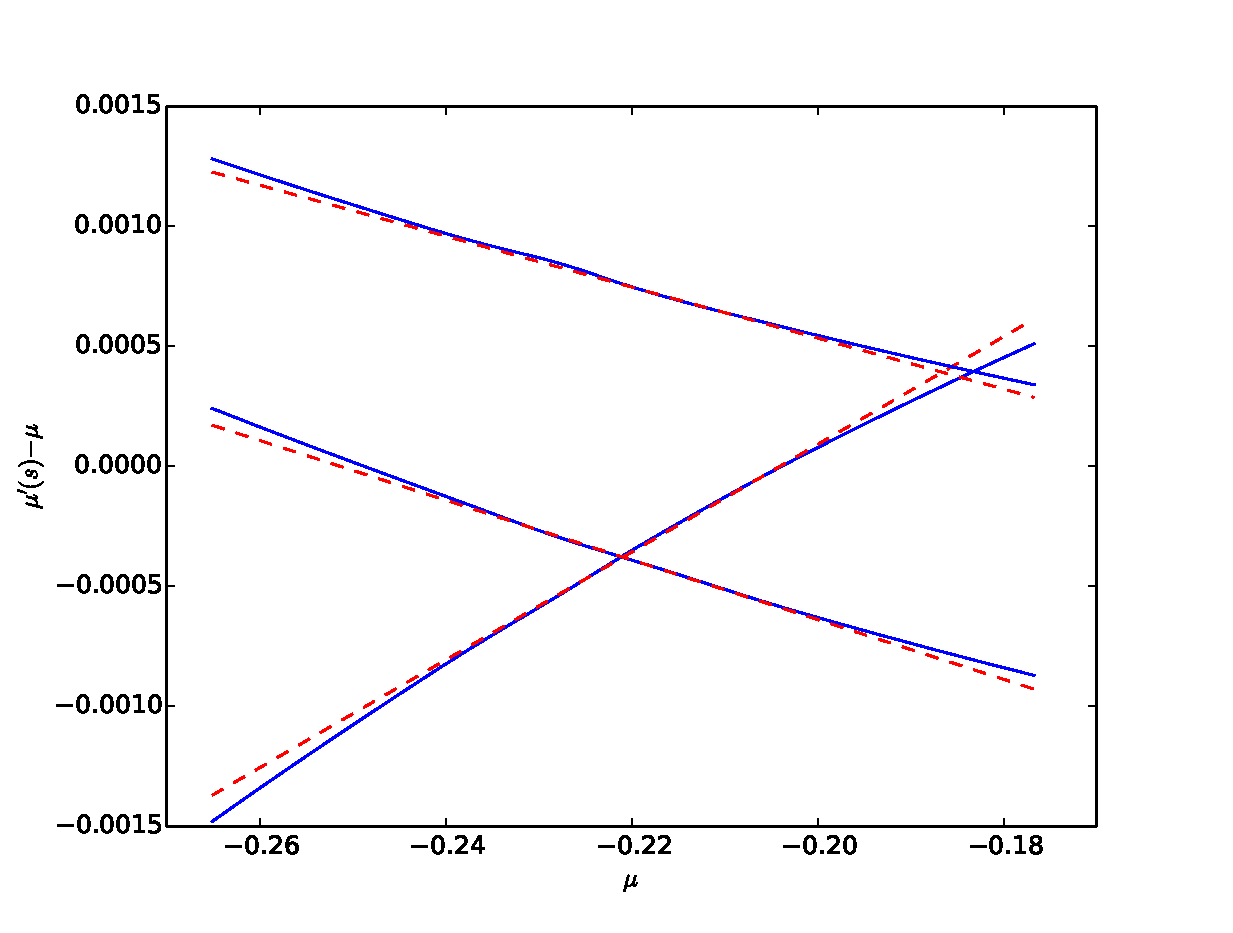
\includegraphics[width = 4.2in]{Images/lin2.eps}
	\end{center}
\end{frame}

\begin{frame}
	\begin{center}
		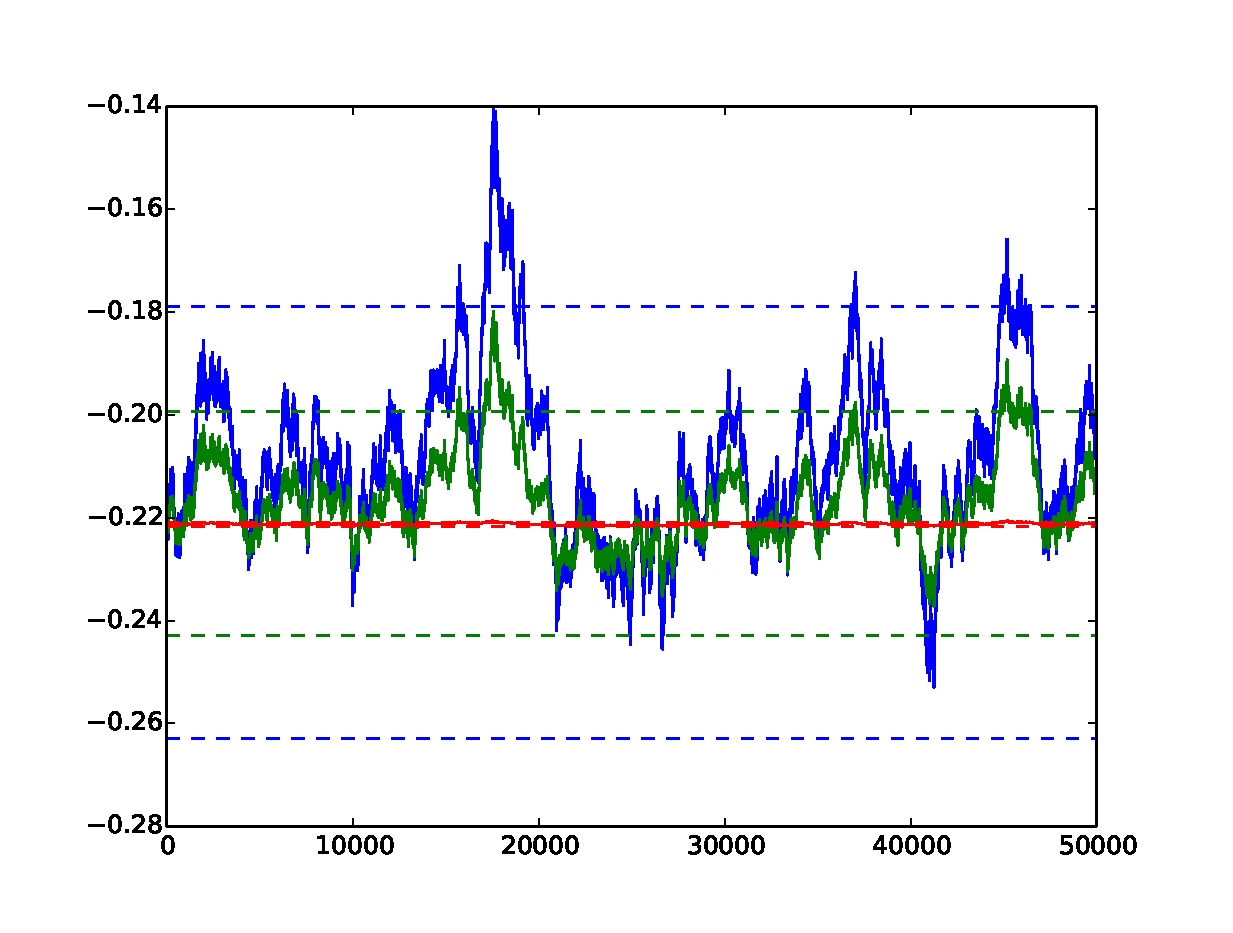
\includegraphics[width = 4.2in]{Images/ErgodicBounds.eps}
	\end{center}
\end{frame}
\end{document}
